\documentclass[journal,12pt,onecolumn]{IEEEtran}
\usepackage[utf8]{inputenc}   % Codificación de entrada
\usepackage[T1]{fontenc}      % Codificación de fuente
\usepackage[spanish,es-tabla]{babel}   % Idioma español
\usepackage{lmodern}          % Fuente moderna
\usepackage{amsmath, amssymb} % Matemáticas y símbolos
\usepackage{graphicx} 		  % Gráficos e imágenes
\graphicspath{{img/}{tablas/}{portada/}}  % Las imágenes se buscarán en la carpeta "img"
\usepackage{longtable}      % Para tablas que se extienden en varias páginas
\usepackage{tabularx}	% Tablas avanzadas
\usepackage{threeparttable}
\usepackage{hyperref}	% Hipervínculos

%-------------------------------------------
% Otros paquetes útiles (personaliza según tus necesidades)
%-------------------------------------------
\usepackage{caption}
\usepackage{subcaption}
\usepackage{xcolor}
\usepackage{setspace}

%-------------------------------------------
% Comandos personalizados
\renewcommand{\listtablename}{Índice de tablas}
\renewcommand{\appendixname}{Anexos}
\definecolor{colorreferences}{RGB}{48,134,3}

% Metadatos del PDF
\hypersetup{
	unicode=true,
	hidelinks,
	colorlinks=true,       % false: boxed links; true: colored links
	linkcolor=black,          % color of internal links (change box color with linkbordercolor)
	citecolor=colorreferences,        % color of links to bibliography
	filecolor=magenta,      % color of file links
	urlcolor=blue,           % color of external links
	linkbordercolor={0 0 0}
}
%-------------------------------------------
% Inicio del documento
%-------------------------------------------
\begin{document}

% Aquí se encuentra el archivo con la portada
\begin{titlepage}
	\centering
	%-------------------------------------------
	% Logos en una tabla: izquierda, centro y derecha
	\begin{tabular}{@{}p{0.3\textwidth} p{0.3\textwidth} p{0.3\textwidth}@{}}
		
\includegraphics[height=2cm]{tecnm} & 
		\centering 
\includegraphics[height=1.5cm]{SEP} & 
		\raggedleft 
\includegraphics[height=2cm]{ith.jpg} \\
	\end{tabular}
	
	\vspace{2em}
	
	\noindent
	%-------------------------------------------
	%	Información institucional y académica (esquina superior izquierda)
	\begin{minipage}[t]{0.48\textwidth}
		\raggedright
		\small \textbf{%
			Instituto Tecnológico de Hermosillo\\
			Materia: Robótica\\
			Profesor: Medina Gil Lamadrid, Jesús Iván%
		}
	\end{minipage}%
	\hfill
	%	fecha actual (esquina superior derecha), en letras pequeñas y en negrita.
	\begin{minipage}[t]{0.48\textwidth}
		\raggedleft
		\small \textbf{\today}
	\end{minipage}
	
	\vspace{2em}
	
	%-----------------------------------------
	% Unidad y Título de la tarea en letras grandes y en negrita
	{\large \textbf{Unidad 1: Morfología del robot}}\\
	{\Huge \textbf{Investigar sobre diferentes tipos de sensores}}
		
	\vspace{1em}
	
	%---------------------------------------
	% Tabla con la información del equipo
	%---------------------------------------
	% Encabezado del equipo
	\begin{center}
		{\Large \textbf{Equipo 4}}
	\end{center}
	
	\vspace{1em}
	
	% Tabla de integrantes:
	% Cada fila contiene: foto (columna izquierda) y datos del integrante (columna derecha)
	\begin{center}
		\begin{tabular}{c c}
			\begin{tabular}{c}
				
\includegraphics[height=3cm]{perfil1.jpg} \\
				\textbf{Fuentes Ochoa},\\ Aislinn Alicia \\ \texttt{l21330583@hermosillo.tecnm.mx} \\ Teléfono: 6371147080
			\end{tabular} &
			\begin{tabular}{c}
				
\includegraphics[height=3cm]{perfil2.jpg} \\
				\textbf{Gonzalez Cueto,}\\ Alejandra Abigail \\ \texttt{l21330591@hermosillo.tecnm.mx} \\ Teléfono: 6221223887
			\end{tabular} \\ \vspace{2em}
			\begin{tabular}{c}
				
\includegraphics[height=3cm]{perfil3.jpg} \\
				\textbf{Ceballos Portillo,}\\ Patsy \\ \texttt{l21330551@hermosillo.tecnm-mx} \\ Teléfono: 6622968916
			\end{tabular} &
			\begin{tabular}{c}
				
\includegraphics[height=3cm]{perfil4.jpg} \\
				\textbf{Peña Encinas}\\ Ana Lourdes \\ \texttt{l21331075@hermosillo.tecnm.mx} \\ Teléfono: (6621281812)
			\end{tabular}
		\end{tabular}
	\end{center}

\end{titlepage}

%	Es innecesario poner el índice porque ya aparece en los marcadores del PDF
\tableofcontents
\newpage

% Ejemplo de inclusión de una sección (por ejemplo, "introduccion.tex" debe estar en la carpeta "secciones" y se recomienda no usar carácteres especiales (tilde) o espacios)
\section{Robot 3}

\begin{figure}
	\centering
	\includegraphics[width=0.5\linewidth]{img/ROBOT3}
	\caption{Robot 3}
	\label{fig:robot3}
\end{figure}

\section{Robot 4}
\begin{figure}[h]
	\centering
	{%
		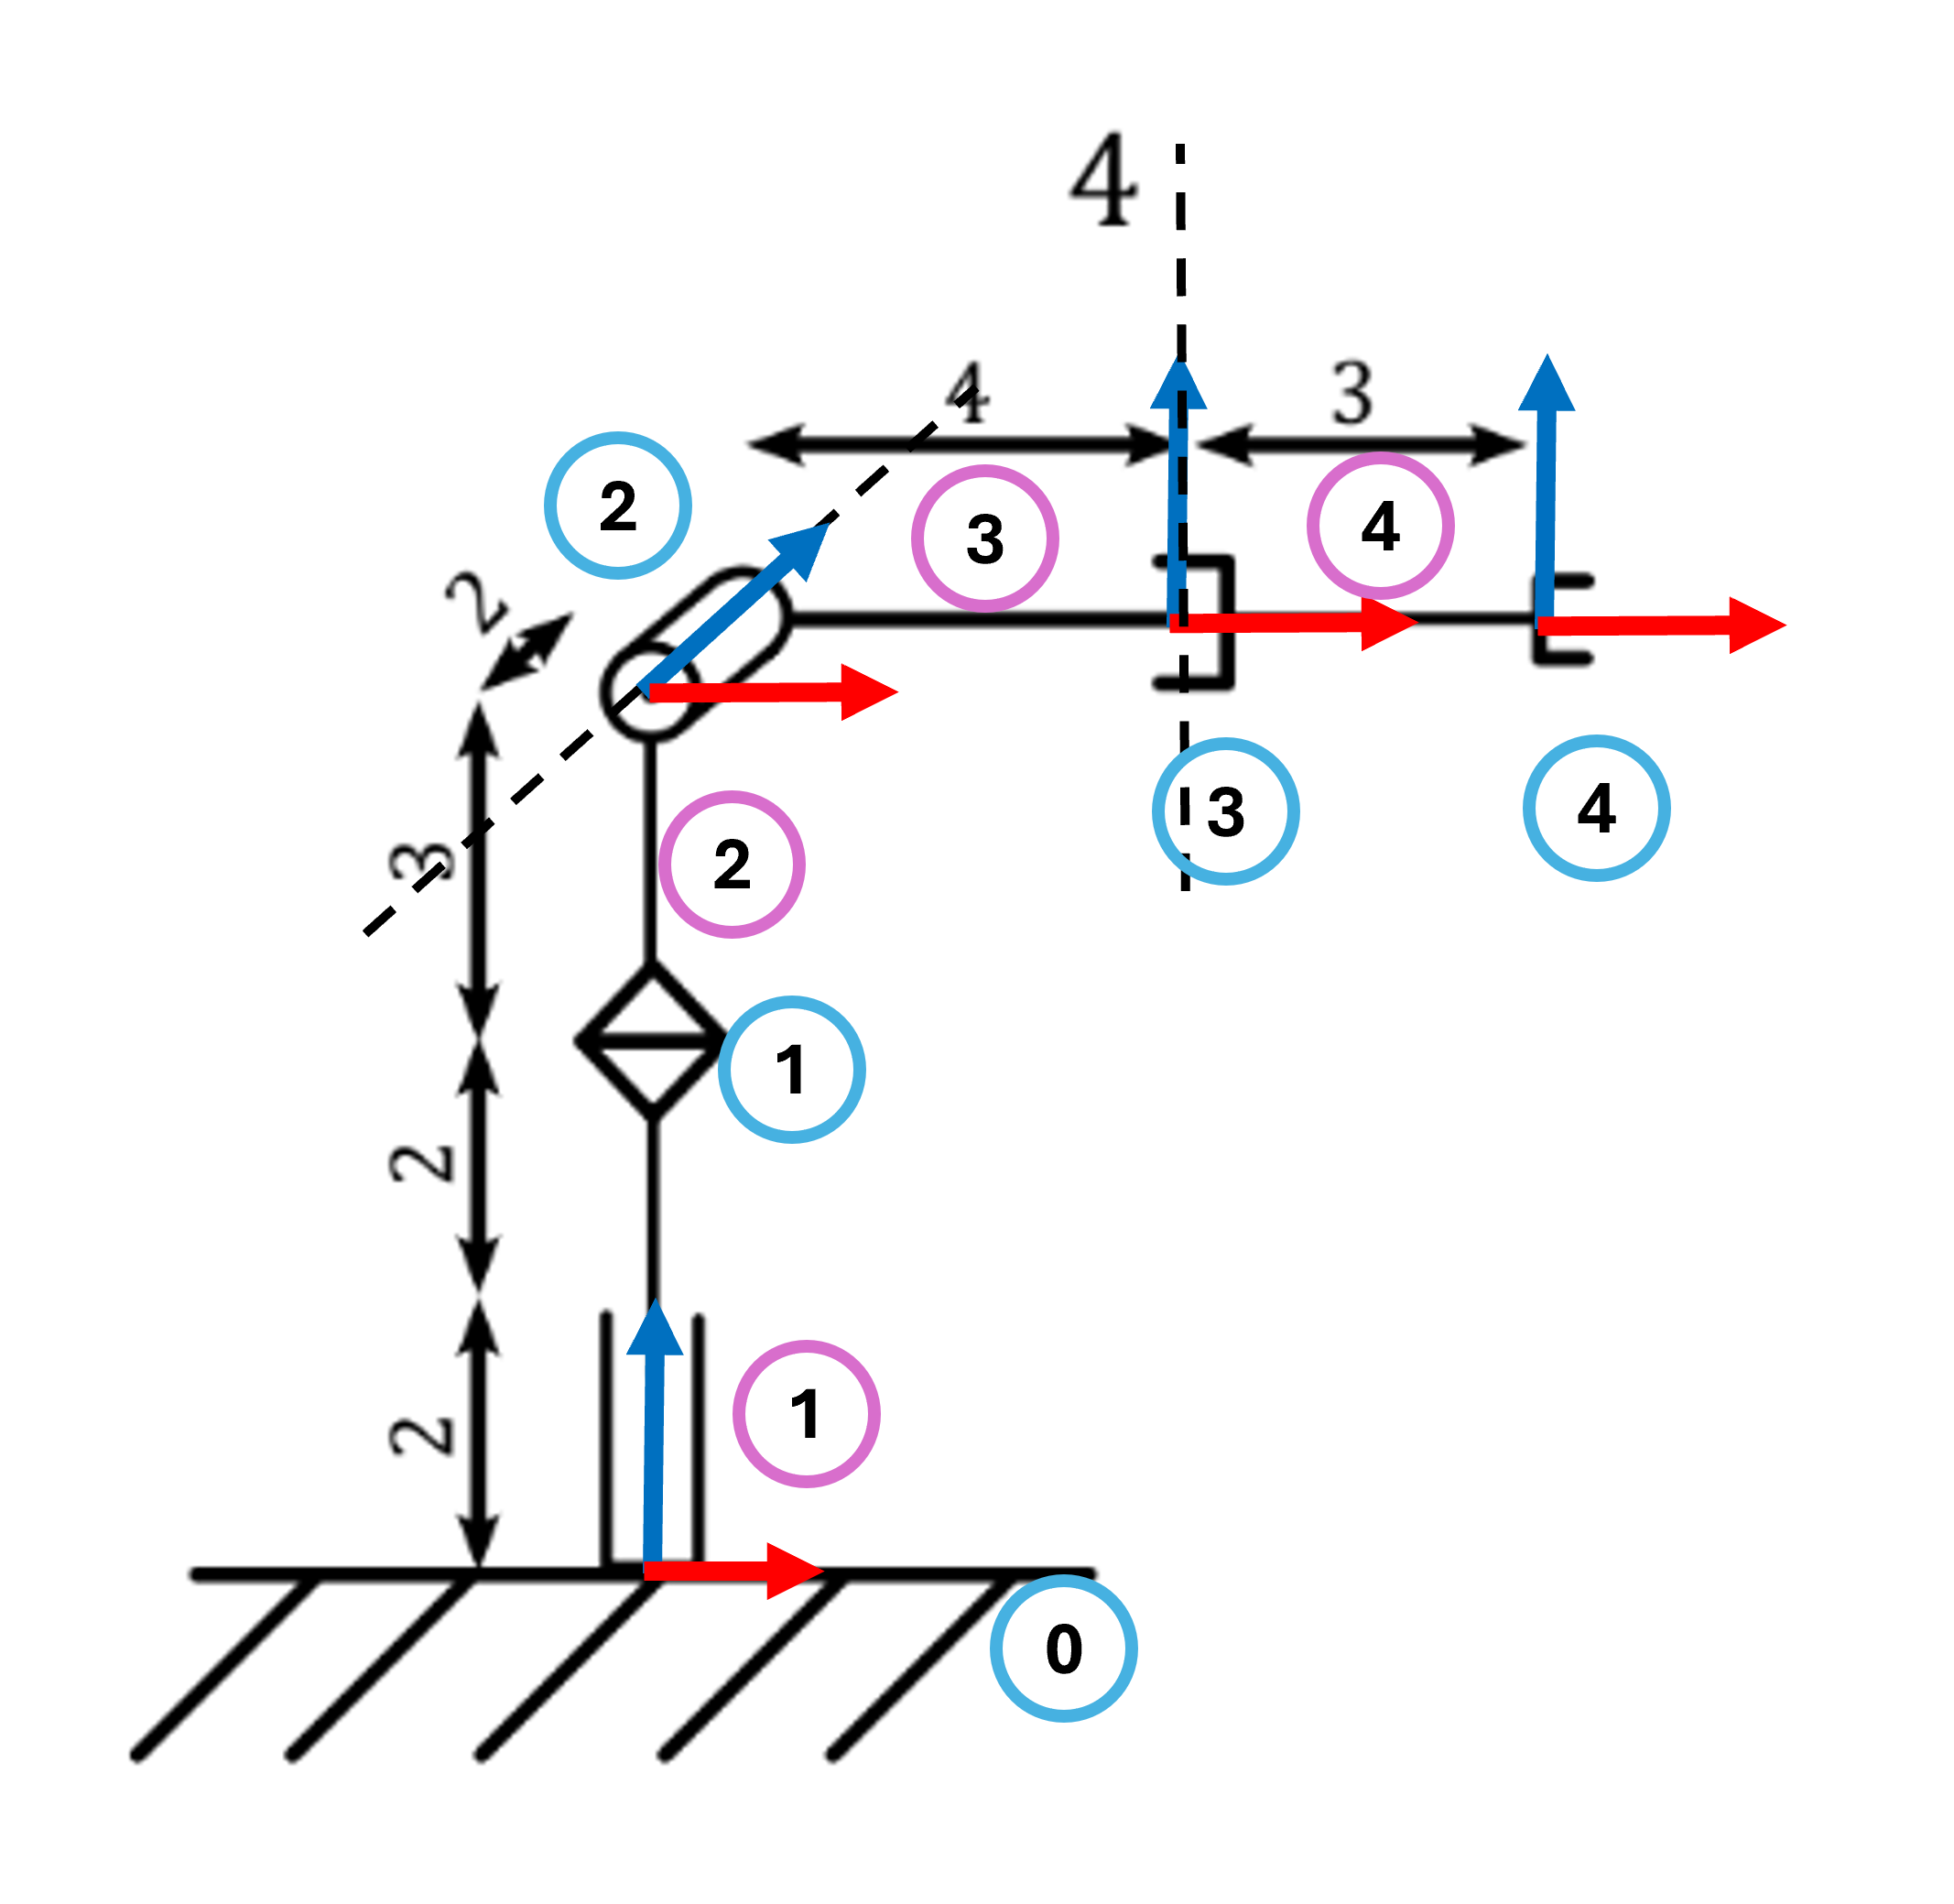
\includegraphics[width=0.7\linewidth]{img/Robot4_1}
		\caption{Robot 4}
		\label{fig:robot41}
	}
\end{figure}
\begin{figure}[h]
	\centering
	{%
		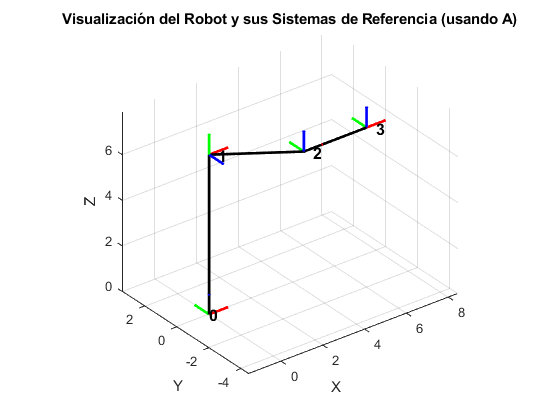
\includegraphics[width=0.7\linewidth]{img/Robot4}
		\caption{Robot 4: Comprobación Matlab}
		\label{fig:robot4}
	}
\end{figure}

\section{Sensores externos} \label{sec:sensores ecternos}
Los sensores externos se dividen en sensores de contacto y sensores sin contacto. 
\subsection{Sensores de contacto}
Son aquellos que necesitan tocar físicamente un objeto para detectar su presencia o medir una magnitud.

\addcontentsline{toc}{subsubsection}{Interruptores de límite}
\subsection*{Interruptores de límite}
\begin{itemize}
	\item \textbf{¿Qué hacen?} Detectan la presencia o posición de un objeto cuando este activa un mecanismo mecánico.
	\item \textbf{Principio de funcionamiento:} Consisten en un brazo mecánico o palanca que, al ser presionado, acciona un interruptor eléctrico.
	\item \textbf{Aplicaciones:} Detección de posición en máquinas CNC y robots industriales.
	Protección en sistemas de seguridad (por ejemplo, cuando una puerta está abierta o cerrada).
	Sistemas de final de carrera en actuadores.
	\item \textbf{Ejemplo:} Interruptor de límite tipo microswitch, como los usados en impresoras 3D para el eje Z.
\end{itemize}
\begin{figure}[h]
	\centering
	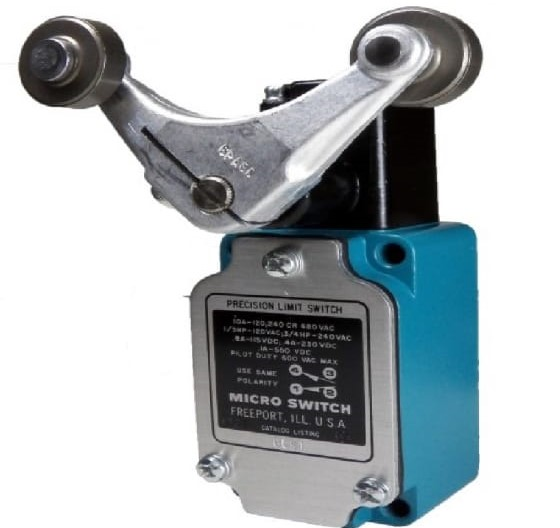
\includegraphics[width=0.3\linewidth]{img/sensor de limite}
	\caption{Sensor de Límite}
	\label{fig:sensor de limite}
\end{figure}

\addcontentsline{toc}{subsubsection}{Interruptores neumáticos}
\subsection*{Interruptores neumáticos}
\begin{itemize}
	\item \textbf{¿Qué hacen?} Detectan la presión de aire o vacío en un sistema neumático.
	\item \textbf{Principio de funcionamiento:} Usan un diafragma o válvula que se activa con cambios de presión.
	\item \textbf{Aplicaciones:} Control en sistemas de automatización neumática.
	Seguridad en prensas neumáticas y sistemas de frenado de emergencia.
	Sistemas de detección de flujo de aire.
	\item \textbf{Ejemplo:} Interruptor neumático utilizado en líneas de producción automatizadas.
\end{itemize}
\begin{figure}[h]
	\centering
	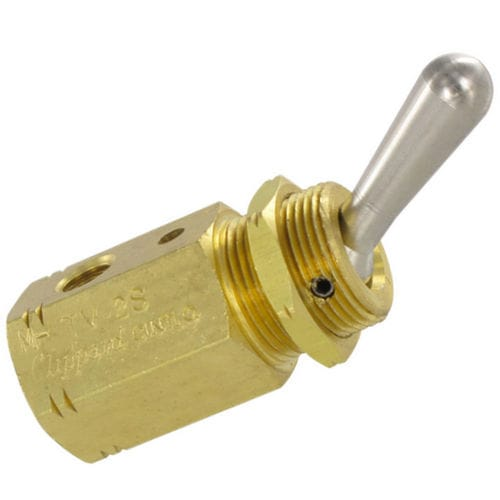
\includegraphics[width=0.2\linewidth]{img/sensor neumatico}
	\caption{Sensor Neumático}
	\label{fig:sensor neumatico}
\end{figure}

\addcontentsline{toc}{subsubsection}{Sensores piezoelectricos}
\subsection*{Sensores piezoeléctricos}
\begin{itemize}
	\item \textbf{¿Qué hacen?} Detectan presión, fuerza o vibraciones y las convierten en señales eléctricas.
	\item \textbf{Principio de funcionamiento:} Se basan en el efecto piezoeléctrico, donde ciertos materiales generan un voltaje al ser sometidos a presión mecánica.
	\item \textbf{Aplicaciones:} Medición de impacto en pruebas de materiales.
	Sensores de vibración en maquinaria industrial.
	Micrófonos y captadores de sonido.
	\item \textbf{Ejemplo:} Sensores piezoeléctricos usados en guitarras eléctricas para captar sonido.
	\cite{carletti_sensores_2025}
\end{itemize}
\begin{figure}[h]
	\centering
	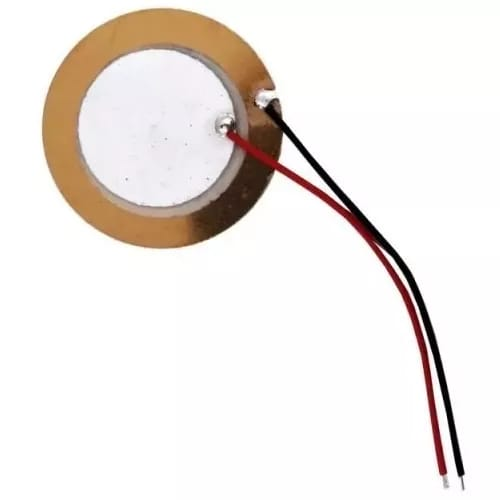
\includegraphics[width=0.2\linewidth]{img/sensor piezoelectrico}
	\caption{Sensor Piezoeléctrico}
	\label{fig:sensor piezoelectrico}
\end{figure}

\addcontentsline{toc}{subsubsection}{Transductores de presión}
\subsection*{Transductores de presión}
\begin{itemize}
	\item \textbf{¿Qué hacen?} Miden la presión de un fluido (líquido o gas) y la convierten en una señal eléctrica.
	\item \textbf{Principio de funcionamiento:} Usan galgas extensométricas o elementos piezoeléctricos para medir la deformación causada por la presión.
	\item \textbf{Aplicaciones:} Monitoreo de presión en sistemas hidráulicos y neumáticos.
	Control de presión en motores y sistemas de refrigeración.
	Aplicaciones médicas (como en esfigmomanómetros digitales).
	\item \textbf{Ejemplo:} Sensor de presión MPX5700 usado en sistemas de control de presión.
	\cite{universalrobots_sensores_robótica}
\end{itemize}
\begin{figure}[h]
	\centering
	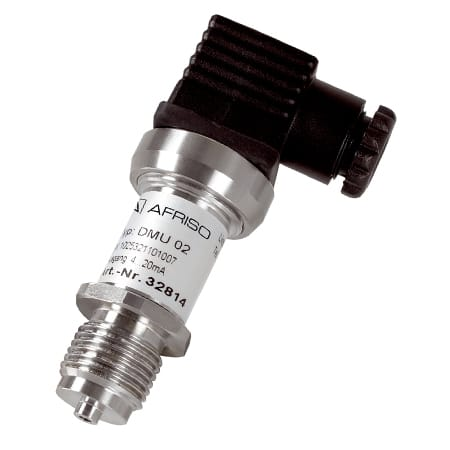
\includegraphics[width=0.2\linewidth]{img/transductor de presion}
	\caption{Transductor de Presión}
	\label{fig:transductor de presion}
\end{figure}
\subsection{Sensores sin contacto}
Detectan la presencia, distancia o características de un objeto sin tocarlo.

\addcontentsline{toc}{subsubsection}{Sensores de proximidad}
\subsection*{Sensores de proximidad}
\begin{itemize}
	\item \textbf{¿Qué hacen?} Detectan la presencia de un objeto cercano sin contacto físico.
	\item \textbf{Tipos y funcionamiento:}
	
	\texttt{Inductivos:} Detectan objetos metálicos mediante un campo electromagnético.
	
	\texttt{Capacitivos:} Detectan objetos metálicos y no metálicos mediante cambios en la capacitancia.
	
	\texttt{Ópticos:} Usan luz infrarroja o láser para detectar objetos.
	\item \textbf{Aplicaciones:} Detección de piezas en bandas transportadoras.
	Sistemas de seguridad en maquinaria.
	Sensores de aparcamiento en automóviles.
	\item \textbf{Ejemplo:} Sensor inductivo LJ12A3-4-Z/BX usado en impresoras 3D.
	\cite{universalrobots_sensores_robótica}
	\cite{robotnik_sensores_2023}
\end{itemize}
\begin{figure}[h]
	\centering
	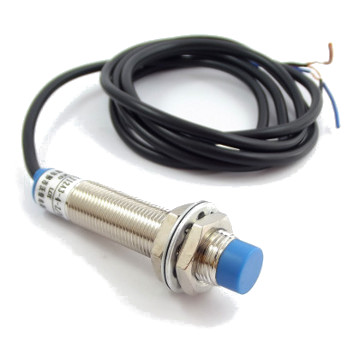
\includegraphics[width=0.3\linewidth]{img/sensor de proximidad}
	\caption{Sensor de Proximidad}
	\label{fig:sensor de proximidad}
\end{figure}

\addcontentsline{toc}{subsubsection}{Sensores de efecto Hall}
\subsection*{Sensores de efecto Hall}
\begin{itemize}
	\item \textbf{¿Qué hacen?} Detectan la presencia de campos magnéticos.
	\item \textbf{Principio de funcionamiento:} Se basan en el efecto Hall, que genera una diferencia de voltaje en un material conductor cuando es atravesado por un campo magnético.
	\item \textbf{Aplicaciones:} Sensores de velocidad en motores.
	Controles de proximidad en robótica.
	Medición de corriente en circuitos eléctricos.
	\item \textbf{Ejemplo:} Sensor de efecto Hall A3144 para detectar imanes.
	\cite{carletti_sensores_2025}
\end{itemize}
\begin{figure}[h]
	\centering
	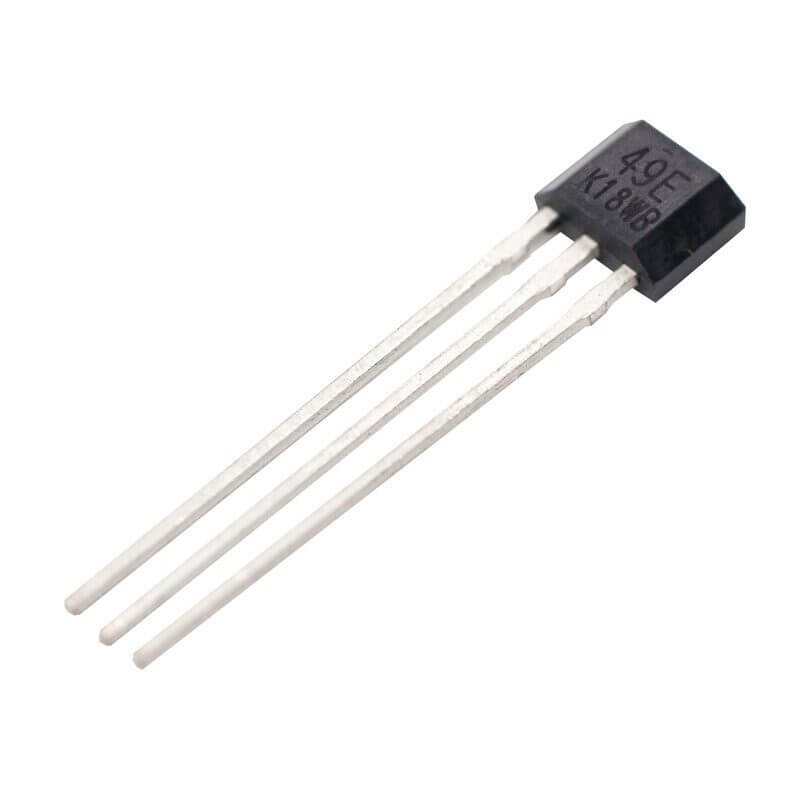
\includegraphics[width=0.2\linewidth]{img/sensor de efecto hall}
	\caption{Sensor de Efecto Hall}
	\label{fig:sensor de efecto hall}
\end{figure}

\addcontentsline{toc}{subsubsection}{Sensores de microondas}
\subsection*{Sensores de microondas}
\begin{itemize}
	\item \textbf{¿Qué hacen?} Detectan movimiento mediante la emisión y recepción de ondas electromagnéticas de alta frecuencia.
	\item \textbf{Principio de funcionamiento:} Utilizan el efecto Doppler: cuando un objeto se mueve, la frecuencia reflejada cambia, lo que permite detectar su presencia y velocidad.
	\item \textbf{Aplicaciones:} Sensores de movimiento en alarmas de seguridad.
	Detección de vehículos en semáforos inteligentes.
	Sensores de radar en autos autónomos.
	\item \textbf{Ejemplo:} Sensor de microondas RCWL-0516 usado en sistemas de iluminación automática.
\end{itemize}
\begin{figure}[h]
	\centering
	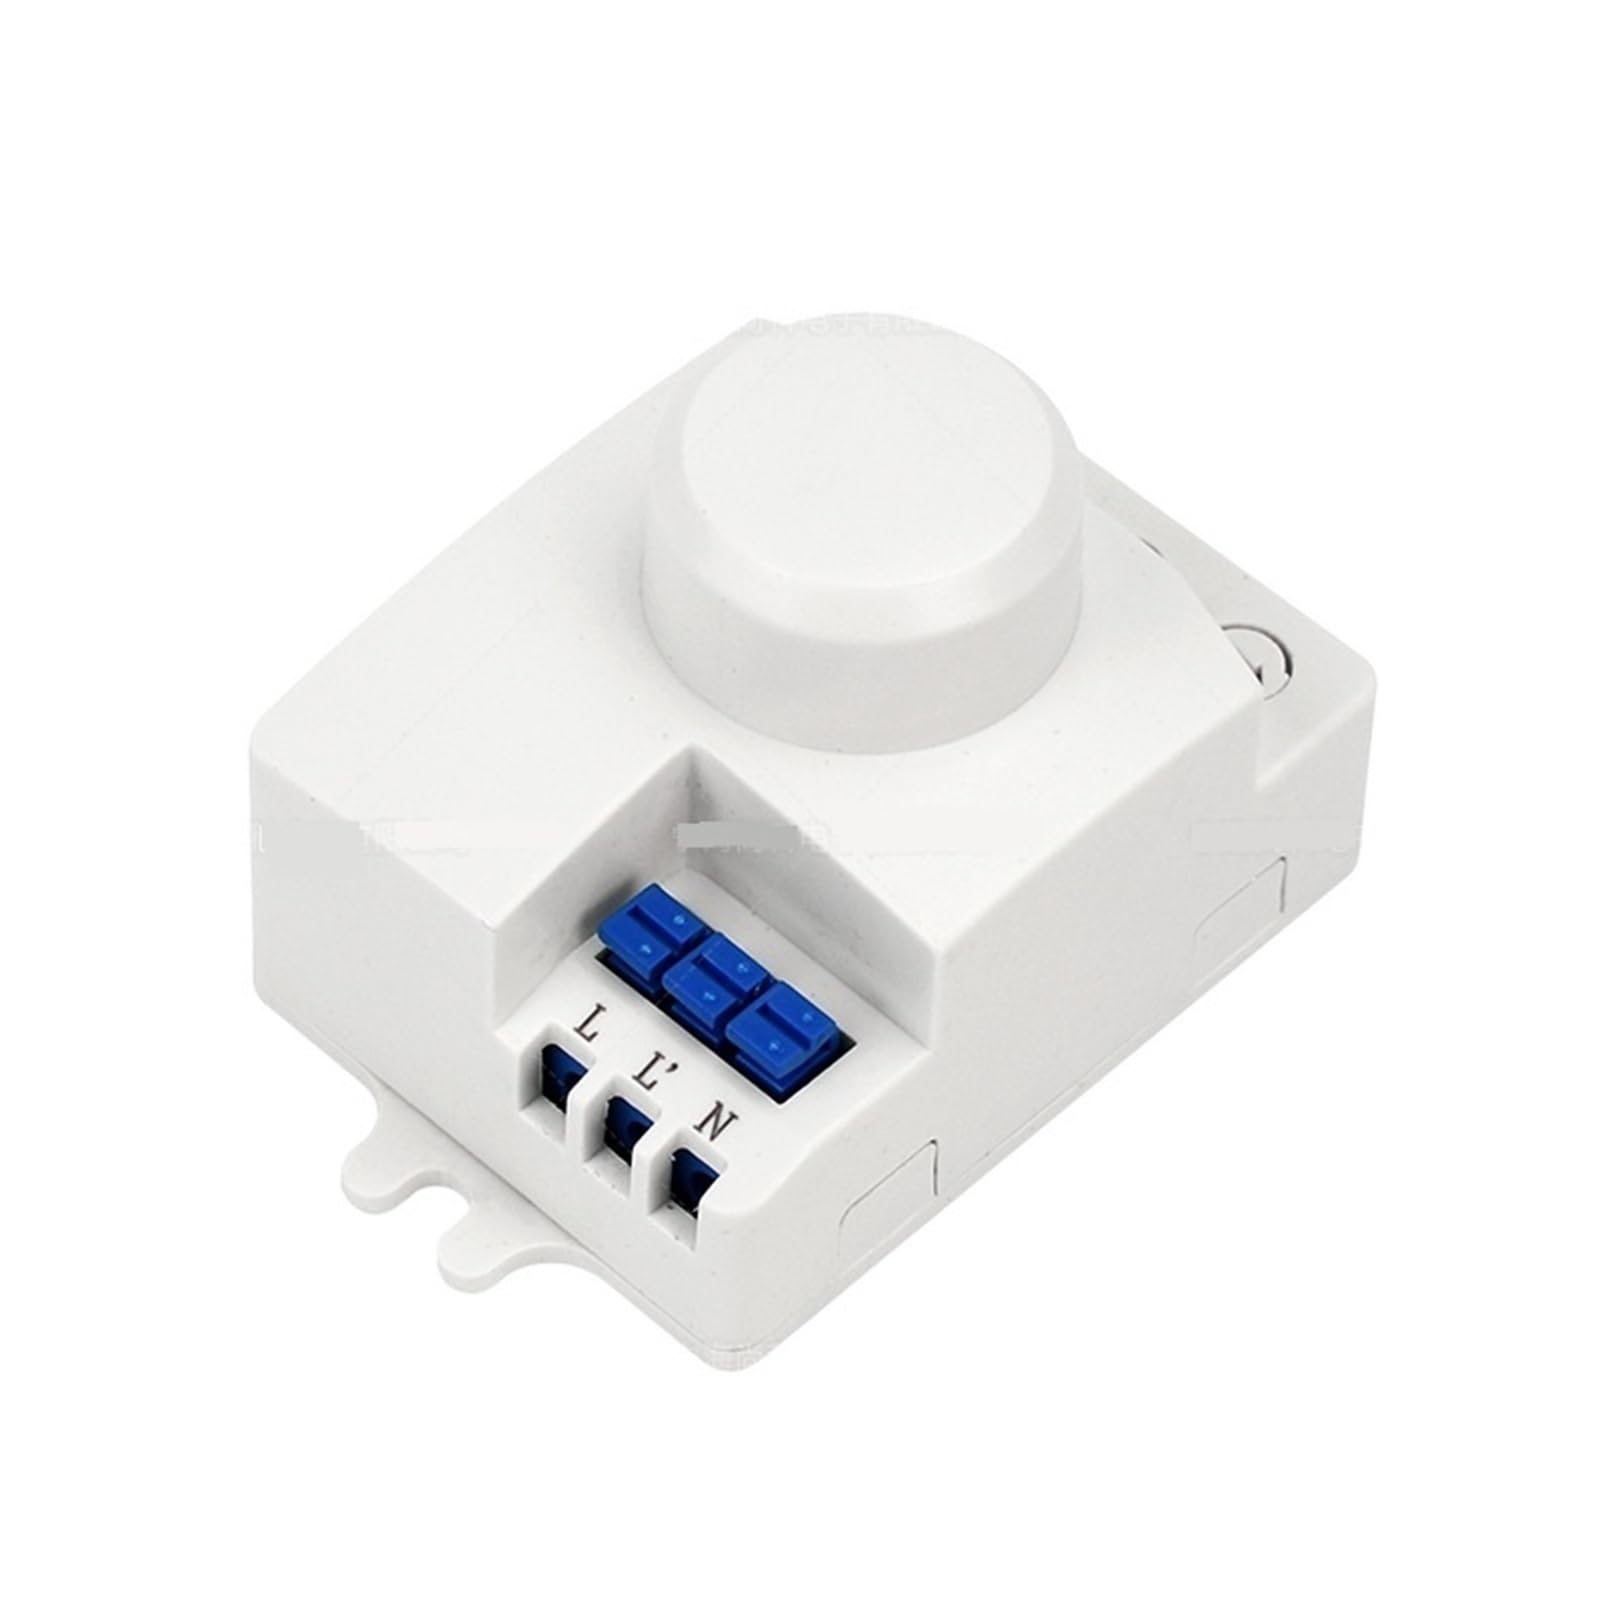
\includegraphics[width=0.3\linewidth]{img/sensor de microondas}
	\caption{Sensor de Microondas}
	\label{fig:sensor de microondas}
\end{figure}

\addcontentsline{toc}{subsubsection}{Sensores ultrasónicos}
\subsection*{Sensores ultasónicos}
\begin{itemize}
	\item \textbf{¿Qué hacen?} Capturan imágenes y procesan información visual.
	\item \textbf{Principio de funcionamiento:} Utilizan cámaras con algoritmos de procesamiento de imagen para detectar formas, colores y movimientos.
	\item \textbf{Aplicaciones:} Inspección de calidad en líneas de producción.
	Reconocimiento facial en seguridad.
	Navegación de robots autónomos.
	\item \textbf{Ejemplo:} Cámara Intel RealSense para visión 3D.
	\cite{makeblock_sensores_2025}
\end{itemize}
\begin{figure}[h]
	\centering
	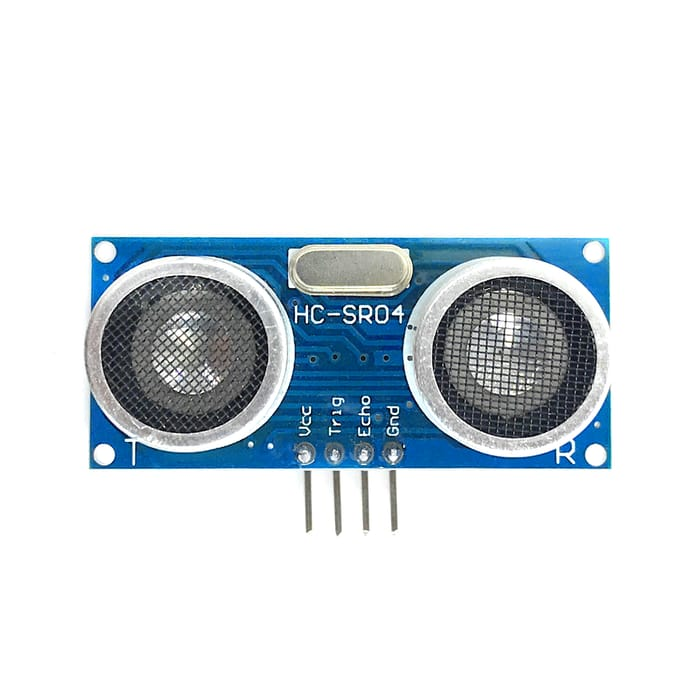
\includegraphics[width=0.3\linewidth]{img/sensor ultrasonico}
	\caption{Sensor Ultrasónico}
	\label{fig:sensor ultrasonico}
\end{figure}

\addcontentsline{toc}{subsubsection}{Sensores láser}
\subsection*{Sensores láser}
\begin{itemize}
	\item \textbf{¿Qué hacen?} Miden distancias con alta precisión mediante un haz de luz láser.
	\item \textbf{Principio de funcionamiento:} Utilizan el tiempo de vuelo (ToF) de un pulso láser para calcular la distancia.
	\item \textbf{Aplicaciones:} Mapeo 3D en drones y vehículos autónomos.
	Medición de distancias en topografía.
	Sensores de seguridad en máquinas industriales.
	\item \textbf{Ejemplo:} Sensor LiDAR TFmini usado en robots para navegación autónoma.	\cite{makeblock_sensores_2025}
\end{itemize} 
\begin{figure}[h]
	\centering
	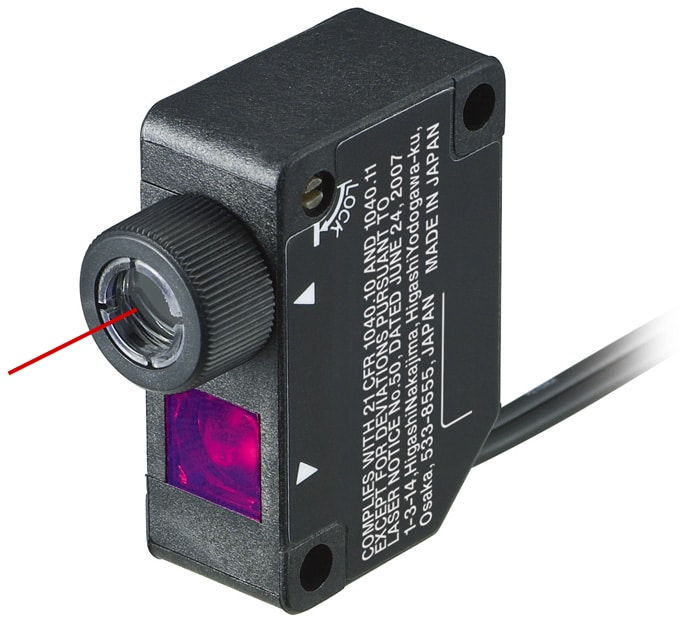
\includegraphics[width=0.3\linewidth]{img/sensor laser}
	\caption{Sensor de Láser}
	\label{fig:sensor laser} 
\end{figure}
\vspace{15cm}
\addcontentsline{toc}{subsubsection}{Sensores de visión}
\subsection*{Sensores de visión}
\begin{itemize}
	\item \textbf{¿Qué hacen?} Detectan movimiento mediante la emisión y recepción de ondas electromagnéticas de alta frecuencia.
	\item \textbf{Principio de funcionamiento:} Utilizan el efecto Doppler: cuando un objeto se mueve, la frecuencia reflejada cambia, lo que permite detectar su presencia y velocidad.
	\item \textbf{Aplicaciones:} Sensores de movimiento en alarmas de seguridad.
	Detección de vehículos en semáforos inteligentes.
	Sensores de radar en autos autónomos.
	\item \textbf{Ejemplo:} Sensor de microondas RCWL-0516 usado en sistemas de iluminación automática.\cite{cognex_vision_sensor}
\end{itemize}
\begin{figure}[h]
	\centering
	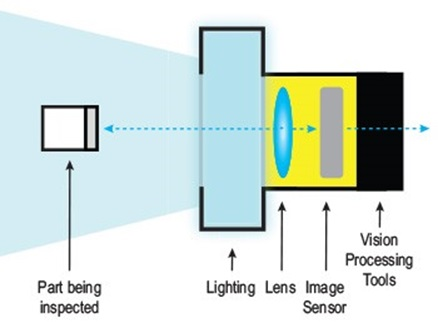
\includegraphics[width=0.3\linewidth]{img/sensor de vision}
	\caption{Sensor de Visión}
	\label{fig:sensor vision}
\end{figure}

\section{Otros sensores}
\subsection*{Giroscopio}
\begin{itemize}
	\item \textbf{¿Qué mide?} La velocidad angular de un objeto en uno o más ejes y se usa para determinar cambios de orientación sin depender de señales externas.
	\item \textbf{Principio de funcionamiento:} Basado en la conservación del momento angular.
	Los giroscopios mecánicos usan un disco giratorio para resistir los cambios de orientación.
	Los giroscopios MEMS (Microelectromechanical Systems) utilizan vibraciones internas y efectos inerciales para detectar movimientos.
	
	\item \textbf{Aplicaciones:} Navegación en drones, aviones y robots autónomos.
	Estabilización en cámaras y dispositivos móviles.
	Sistemas de navegación inercial en submarinos y misiles.
	\item \textbf{Ejemplo:} MPU6050 (combinado con acelerómetro).
\end{itemize}
\begin{figure}[h]
	\centering
	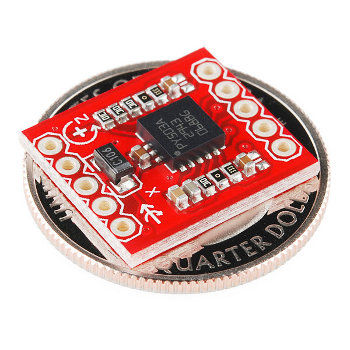
\includegraphics[width=0.3\linewidth]{img/giroscopio}
	\label{fig:giroscopio}
\end{figure}
\subsection*{Acelerómetro}
\begin{itemize}
	\item \textbf{¿Qué mide?} La aceleración lineal en uno o más ejes (X, Y, Z) y puede detectar vibraciones, inclinaciones y fuerzas de impacto.
	\item \textbf{Principio de funcionamiento:} Basado en la segunda ley de Newton: F=maF = maF=ma.
	Los acelerómetros MEMS usan pequeñas masas móviles dentro del sensor que se desplazan con la aceleración, generando una señal eléctrica.
	\item \textbf{Aplicaciones:} Detección de caídas en dispositivos móviles y wearables.
	Control de movimiento en robots y videojuegos.
	Airbags en automóviles (detectan colisiones).
	Análisis de vibraciones en maquinaria industrial.
	\item \textbf{Ejemplo:} ADXL345 (digital, de 3 ejes).
\end{itemize}
\begin{figure}[h]
	\centering
	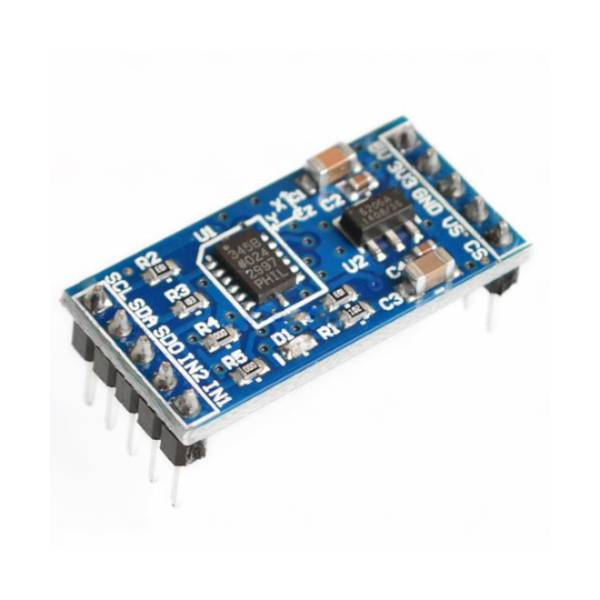
\includegraphics[width=0.3\linewidth]{img/acelerometro}
	\label{fig:acelerometro}
\end{figure}
\subsection*{Magnetómetro}
\begin{itemize}
	\item \textbf{¿Qué mide?} La intensidad y dirección de los campos magnéticos y permite determinar la orientación respecto al campo magnético terrestre (como una brújula digital).
	\item \textbf{Principio de funcionamiento:} Utilizan el efecto Doppler: Utiliza el efecto Hall o materiales magnetorresistivos para detectar cambios en los campos magnéticos.
	Puede detectar objetos metálicos o variaciones en el campo magnético de la Tierra.
	\item \textbf{Aplicaciones:} Brújulas digitales en smartphones y GPS.
	Navegación en vehículos autónomos y drones.
	Detectores de metales.
	Exploración geofísica para medir anomalías magnéticas en la Tierra.
	\item \textbf{Ejemplo:} HMC5883L (popular en drones y navegación).
\end{itemize}
\begin{figure}[h]
	\centering
	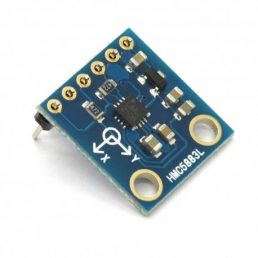
\includegraphics[width=0.3\linewidth]{img/magnetometro}
	\label{fig:magnetometro}
\end{figure}
\subsection*{LiDAR (Light Detection and Ranging)}
\begin{itemize}
	\item \textbf{¿Qué mide?} Distancias a objetos mediante la emisión y recepción de pulsos láser.
	Puede generar mapas en 3D con alta precisión.
	\item \textbf{Principio de funcionamiento:}Emite un pulso de luz láser y mide el tiempo que tarda en reflejarse en un objeto y regresar al sensor.
	\item \textbf{Aplicaciones:} Vehículos autónomos (detección de obstáculos y mapeo).
	Topografía y cartografía en 3D.
	Agricultura de precisión (detección de variaciones en el terreno).
	Arqueología (descubrimiento de estructuras ocultas bajo vegetación).
	\item \textbf{Ejemplo:} Velodyne LiDAR (usado en coches autónomos).
	RPLIDAR A1 (más accesible para proyectos de robótica).
\end{itemize}
\begin{figure}[h]
	\centering
	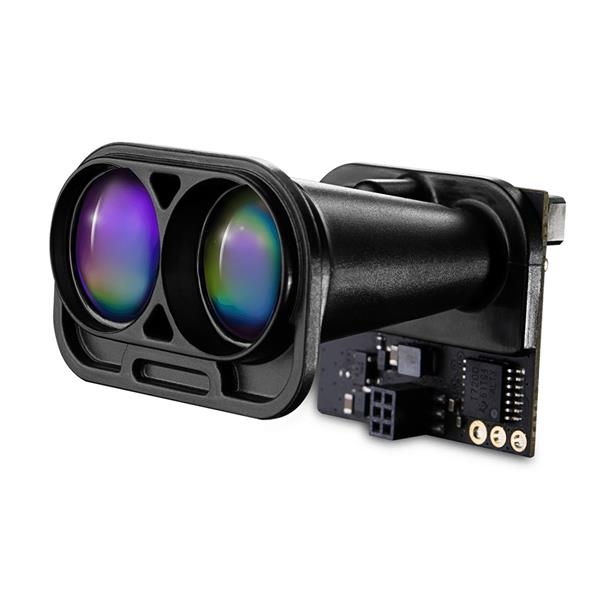
\includegraphics[width=0.3\linewidth]{img/LiDAR}
	\label{fig:LiDAR}
\end{figure}
%\section{Conclusión} \label{sec:conclusion}
%Solo añadan esta sección si lo consideran necesario. No es deben poner un resumen del contenido ni información importante que no se haya mencionado en una sección principal. Pueden poner la parte en la que más batallaron, el conocimiento más importante que consideran haber obtenido o algún comentario.
%\subsection{Persona 1}
%En caso de que haya sido una perspectiva individual, tienen que poner los comentarios de cada integrante y su nombre.
%\subsection{Persona 2}
%Es\part{\label{key}}to me dará una retroalimentación desde la perspectiva de diferentes alumnos con diferentes roles.

%-------------------------------------------
% Bibliografía
%-------------------------------------------
\bibliographystyle{IEEEtran}  % Estilo de bibliografía IEEE
% La bibliografía se tomará del archivo "fuentes.bib"
\bibliography{fuentes}
	
\end{document}
